%%gji_extra_guide.tex

\documentclass[extra,mreferee]{gji}
%\usepackage{timet}

\usepackage{graphicx}
\graphicspath{ {./figures} }
\usepackage{subfig}
\usepackage{caption}
\usepackage{floatrow}
\usepackage{amsmath}
\usepackage{color}
\floatsetup[figure]{style=plain,subcapbesideposition=top}
%\usepackage[margin=70mm]{geometry}

%\usepackage{subfig}

\title[\texttt{gji\_extra.sty} ]  
  {\texttt{GLAD-M25} - global adjoint tomography model} 
  
\author[]  {Wenjie lei, Jeroen Tromp, ...}  

\newcommand{\btx}{\textsc{BibTeX}}

\begin{document}

\maketitle

\section{Introduction}
With the development of high performance computing and numerical methods, it is now possible to using adjoint method to image the interior the globe using thousands of earthquakes. 

There are few agreements about the earth model and yet many unknown to be resolved. There are quite a lot of global models exits however there is no such con-sense. 

The GLAD-M25 is the first earth model that incorporate the P and S wave speed using full waveform inversion. Also, people are using specific set of phases in their inversion. For P models, people are using P phase and other body wave phases and for S models, people are using mostly S wave phases and surface waves to constrain the structure. Those two kinds of models usually reveals very different parts of the earth. For example, for P wave, people used it the image the subduction slabs and it is not very good at image lower mantle structures, such as plumes and lower mantle convections. For S waves, it is the verse verso.

There are many challenges coming along the way. First, the data volume is huge.  There are in total of 1480 earthquakes used in the inversion stage, added into the database step by step. Second, workflow management is crucial dealing with such a large project. One factor is coming from the complex workflow. There are 4 major building blocks, forward simulation, seismic data processing, adjoint simulation and post-processing. Each blocks contains several small blocks. The other factor is coming from the number of earthquakes and high demands of computation. In each iteration, we are doing 1480 forward and adjoint simulation, generating a few Petabyes of wavefiled files and consuming 16 million of CPU hours on the supercomputer at Oak Ridge National Lab. There are yet more in data processing stages. How to deal with hardware failures is very important and prevent containmination into our inversion results.

Here, we present our GLAD-M25 earth model, with significantly improvements on the plumes and subductions.


\section{Starting Model}

We used GLAD-M15 as our starting model. The GLAD-M15 is a 3D transverslty isotropic earth model which uses S362ani + CURST2.0 as its own starting model. It then uses 256 earthquakes and broad-band seismic data to do the 3D full-waveform inversion\cite{Ebru2015}. It uses 15 conjugate graident iterations to update the crust and mantle. The first 12 iterations of GLAD-M15 was performed under 27 secs and the last 3 under ~17 secs. In our inversion, we use the 17s resolution.

It provides 6 model parameters, mass density($\rho$), two compressional wavespeeds($\alpha_v$ and $\alpha_h$), tws shear wavespeeds($\beta_v$ and $\beta_h$) and a dimenionless parameter($\eta$). We will discuss the model parametrization in detail in the following sections.

\section{Earthquakes}
We selected 1040 earthquakes from Global CMT catalog. The mangitudes ranges from 5.5 to 7.0. The lower band is set to ensure the signal-to-noise ratio at the global scale. The upper bound of magnitude, 7.0, is set because the minimal period of waveform is 17s. We also constrain the duration of CMT sources to be smaller than 17s.

We carefully inverted the source mechanism using our starting model, GLAD-M15. The seismic data was filtered into 50-100s to select body wave windows and 60-100s to select surface wave windows\cite{globalCMT}. The inverted parameters includes moment tensors, longitude, latitude and depth. A grid search for the scalar moment and origin time correction was applied directly after the waveform-type of inversion to future calibrate the sources since the first stage inversion algorithm is not very sensitive to those two parameters.
On average, we observed ** km change in depth and ** km change in location. The moment tensor is not changed dramatically and the Global CMT provides good enough focal mechanism. The scalar moment, on the average, has **\% change.

In our 1st iteration, we used 520 earthquakes, as the first iteration is mainly to test our tools, to make sure software are robust and scalable. Starting from 2nd iteration, we double the number of earthquakes, further expanding our dataset to 1040 earthquakes. Starting from GLAD-M22, we added 440 earthquakes from GLobal CMT catelog, mainly in previously poorly covered regions. However, due to computational cost, we didn't implement the 1st stage source inversion in the newly added 440 earthquakes but only calibrate its origin time and scalar moment.

include the earthquake map here.

\begin{figure}
\includegraphics[width=\textwidth]{figures/events_1480.pdf}
\caption{1480 earthquakes used in this study. (a) Distribution of earthquakes The color of beach ball denotes the depth range of earthquakes from Global CMT Catalog \cite{GlobalCMT}. {\color{Blue}Blue} is for shallow earthquake which are above 50km, {\color{Green}Green} is between 50 and 300km and {\color{Red}Red} is below 300km.}
\centering
\end{figure}

\section{Seismic Data}

Seismic stations have been very carefully picked to ensure global converage and high data quality. There are global seismic networks which provides good global coverage, such as the Global Sesimic Netowork(GSN), GEOFON, GEOSCOPE. Regional networks, on the other hand, also becomes a significant part in our database and greatly improve the ray coverage at specific regions, such as US Array(TA), Africa Array(AF), Canadian National Seismograph Network (CN), Geoscience Australia (AU), Brazilian Lithospheric Seismic Project (BL), Antarctic Seismographic Argentinean Italian Network (AI), Caribbean Network (CU), the New Zealand National Seismograph Network (NZ) and etc. There are in total of *** seismic networks and 10,000 seismic stations used in our inversion.

The data, associated with the earhtquakes, was downloaed from several data centers, including IRIS, ORFEUS, INGV, IPGP, ETH, GEONET, RESIF, GFZ and BGR. We only include broad-band seimometers and there in total of 10,000 seismic stations occurred in our database.

include the station map here...

\begin{figure}
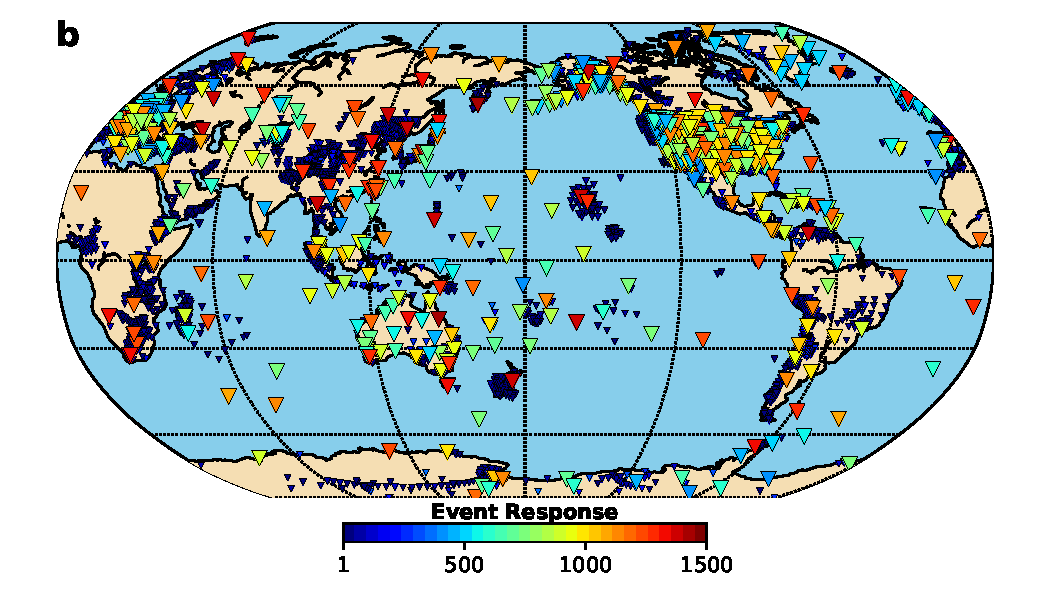
\includegraphics[width=\textwidth]{figures/station_map.pdf}
\caption{Locations of 1480 earthquakes used in this study.}
\centering
\end{figure}

\section{Misfit function and Model Parametrization}

\begin{table}[!htb]
\caption{Measurement Categories. Seismic waves are categorized in terms of complementary period bands on three components of motion.}
\label{tab:category}
\begin{tabular}{|c|c|c|c|}
\hline
~          &  Vertical & Radial &  Transverse \\
\hline
17--40~s   &   P-SV body waves          & P-SV body waves           & SH body waves   \\
40--100~s  &   P-SV body waves          & P-SV body waves           & SH body waves \\
40--100~s  &   Rayleigh mantle waves    & Rayleigh mantle waves     & Love mantle waves \\
90--250~s  &   Rayleigh surface waves   & Rayleigh surface waves    & Love surface waves \\
\hline
\end{tabular}\\
\label{table:categories}
\end{table}

\begin{table}[!htb]
\caption{Misfit Reduction from M00 to M25 for 1480 earthquakes used in the inversion}
\label{tab:category}
\begin{tabular}{|c|c|c|c|}
\hline
~          &  Vertical(\%) & Radial(\%) &  Transverse(\%) \\
\hline
17--40s                &   31.1    &       37.1 &       42.2 \\
40--100s body waves    &    31.3   &       40.2 &       42.0 \\
40--100s surface waves &   50.1    &       51.1 &       53.8 \\
90--250s               &    36.2   &       38.8 &       38.6 \\
\hline
\end{tabular}\\
\label{table:categories}
\end{table}

\begin{table}[!htb]
\caption{Misfit Reduction from M00 to M25 for 360 earthquakes as held-out dataset}
\label{tab:category}
\begin{tabular}{|c|c|c|c|}
\hline
~          &  Vertical(\%) & Radial(\%) &  Transverse(\%) \\
\hline
17--40s                &         29.2 &       33.7 &       43.4 \\
40--100s body waves    &         26.2 &       32.2 &       39.0 \\
40--100s surface waves &         49.1 &       49.4 &       51.2 \\
90--250s               &         30.9 &       34.8 &       34.9 \\
\hline
\end{tabular}\\
\label{table:categories}
\end{table}

\begin{table}[!htb]
\caption{Misfit Reduction from M15 to M25 for 1480 earthquakes used in the inversion}
\label{tab:category}
\begin{tabular}{|c|c|c|c|}
\hline
~          &  Vertical(\%) & Radial(\%) &  Transverse(\%) \\
\hline
17--40s                &   17.4   &       21.1 &       24.6 \\
40--100s body waves    &   16.8   &       21.3 &       21.7 \\
40--100s surface waves &   28.5   &       28.3 &       28.4 \\
90--250s               &     14.5 &       13.4 &       25.7 \\
\hline
\end{tabular}\\
\label{table:categories}
\end{table}



\begin{table}[!htb]
\caption{Misfit Reduction from M15 to M25 for 360 earthquakes as held-out dataset}
\label{tab:category}
\begin{tabular}{|c|c|c|c|}
\hline
~          &  Vertical(\%) & Radial(\%) &  Transverse(\%) \\
\hline
17--40s                &          11.8 &       14.1 &       21.5 \\
40--100s body waves    &          14.5 &       12.9 &       16.9 \\
40--100s surface waves &          29.3 &       28.1 &       23.7 \\
90--250s               &          10.9 &       14.3 &       24.0 \\
\hline
\end{tabular}\\
\label{table:categories}
\end{table}

The overall misfit, $\Phi$, is defined as follows:

\begin{align}
\label{eq:misfit}
\Phi = \sum_{s}^{S} \omega_s \sum_{c}^{C} \omega_{c} \sum_{r}^{R_{sc}} \omega_{scr} \sum_{w}^{N_{scr}} \omega_{scrw}\, \chi_{scrw}
\quad ,
\end{align}\\
where~$S$ denotes the number of sources, $C$ the number of categories,
$R_{sc}$ the number of receivers for source~$s$ and category~$c$, and~$N_{scr}$ the number of measurements for source~$s$,
category~$c$ and receiver~$r$.
The misfit for source~$s$,
category~$c$, receiver~$r$, and window~$w$ is
\begin{align}
\chi_{scrw} = \left(\frac{\Delta m_{scrw}}{\sigma_{scrw}}\right)^2
\quad ,
\end{align}
where~$\Delta m_{scrw}$ denotes a measurement with associated standard deviation~$\sigma_{scrw}$.-

\subsection{Weightings}
Weighting is crucial to the global tompgraphy. Since most of the earthquakes happen in the in the plate boundaries and most of the seismic stations located in the continents(mostly in the northern hemisphere). Also, there are very dense seismic arrays, such as US array, deployed recently. All the factors mentioned above will lead to a really unevent distribution of ray paths. Our weighting strategy is developed to compensate such effects.

Our weighting algorithm is used to determine the $\omega_{scr}$ and $\omega_s$. $\omega_{scr}$ is the receiver weightings given one source and one category and $\omega_s$ is the source weighting based on it locations. Both problems can be simplied as: given the distrubtion of points in the space to determine the weighting asssociated with each point. Here we introduce the exponential weightings to describe the density of points and mimic the behavior of point correlations.

For more details for the weightings, please refer to the Appendix.

\subsection{Model parametrization}

Transversly isotropy model parametrization is used in our model, which is the same as GLAD-M15. Compared to a general anisotropic model which has 21 independent variables, our model could be described by 5 Love parameters,  A, C, L, N and F. In seismology, it is more straight forward to define the parameter with regarding to wavespeed. Instead of Love parameters, we have $\alpha_v$, $\alpha_h$, $\beta_v$, $\beta_h$ and $\eta$. The parameters can be further reduced to 4 assuming the radial anisotropy is due to shear anistropy, we introduced the buld sound speed, $c=\sqrt{\kappa/\rho}$. Our final parameters is:\\
\begin{align*}
c &= \sqrt{\kappa/\rho} \\
\beta_v &= \sqrt{L/\rho} \\
\beta_h &= \sqrt{N/\rho} \\
\eta & = F/(A-2L)
\end{align*}

The density is hard to contain in our study due to the period band we are working on. So it is constrained by isotropic shear wavespeed, $\beta = \sqrt{(2\beta_v^2 + \beta_h)/3}$,\\
\begin{equation*}
    \delta ln\rho = 0.33\delta ln\beta
\end{equation*}

Based on the parametrization described above, the perturbations in misfit functions would be:

\begin{equation*}
    \delta \chi = \int_V (K_c\delta lnc + K_{\beta_v}\delta ln\beta_v + K_{\beta_h}\delta ln\beta_h + K\eta \delta ln\eta) dV 
\end{equation*}

\section{Adjoint Tomography Workflow}

\subsection{Forward simulation}
The forward simulation takes the CMT sources, stations and Earth models as input. It will generate synthetic seismograms and forward wavefield snapshots. We used SPECFEM3D-GLOBE as the software to calculate the sysnthetic seismograms with GPU acceleration on Titan at the Oak Ridge Nation Lab.

We simulate 120min of seismigrams. It taks 384 Tesla K20 GPUs approximately 10 mins to do the simulation on Titan at the Oak Ridge National Lab for each earthquakes. To fully undo the attenuation, there is also forward wavefiled saved to the disk. In out current 17sec resolution and 120min simulation, for each earthquake, the forward wavefiled is about 1TB. Given the size the 1480 earthquakes, we have 1.5TB of wavefiled during about 10 hours's of simulation, which is huge volume of I/O happening during the calculation.

\subsection{Seismic Data Processing}

The seismic data processing takes the raw observed and synthetic data as input, and generate s the adjoint sources as the output. The preprocessing includes: 1) signal processing that  filter into different period bands and rotate the seismograms from East and North to Radial and transverse.; 2) window selection that pick the time window on a pair of observed and synthetic seismigrams; 3) frequency-dependent measurement that generate travel-time measurements inside the windows; 4) measurements quality checks that throw out bad windows and associated measurements and only keep good ones; 5) calcualte the adjoint sources; 6) for each window calculate its weightings that will be applied to the overall misfit function; 7) construct the final adjoint sources by combining the measurements in different period bands.

\subsection{Adjoint Simulation}
The adjoint simulation takes the adjoint sources as input, and calculate the Frechet derivatives as output. The computation cost is twice as the forward simulation since it is both calculating the adjoint wavefiled and reconstruct the forward wavefield. Other than the adjoint sources, the adjoint simulation also reads in the saved forward wave. 

The Adjoint simulation nows takes about 20 mins for 17sec resolution and 120min simlulation, which about the twice the time of forwards simulation, since it needs to calculate both a forward and adjoint wavefield at the same time.

\subsection{Post-processing}
The post-processing takes the Frechet derivatives as the input and generate the model updates as the output. It contains: 1) summation of single event kernels; 2) smoothing the summed kernels; 3) Preconditions using pseudo-Hessian; 4) Numerical optimization to get serach direction; 5) calculate the step length on the search direction; 6) update the model using the search direction and step length.

Conjugated gradient methds was used from M00 to M21. Then L-BFGS was used afterwards. Here we will discuss the L-BFGS methods in details.

\subsubsection{L-BFGS}

Assuming the model is $m_i$ and gradient is $g_i$ at iteration i, we defined the change of model and gradient:\\
\begin{equation*}
    \Delta m_i = m_{i+1} - m_i \quad
    \Delta g_i = g_{i+1} - g_i
\end{equation*}

and \\
\begin{equation*}
     \rho_k = \frac{1}{\Delta g^{T} \Delta m}
\end{equation*}

The L-BFGS iteration could be described below, at iteration k \cite{NumericalOptimization}:

\begin{align*}
q = g_i \\
for \quad i = k -1, k-2, ..., k-n \\
\alpha_i = \rho_i \delta_m_i^{T}q \\
q = q - \alpha_i \delta g_i \\
end for\\
r = H_k^{0}q \\
for i = k-n, k-n+1, ..., k-1 \\
\beta = \rho_i \delta g_i^{T}r \\
    r = r + \delta m_i(\alpha_i - \beta) \\
end for \\
\end{align*}

The search direction for L-BFGS is:
$$d_i = -r$$

The step length is choosen based upon line search along the search direction of the overall misfit function. 

\subsection{Adapative Seismic Data Format}

It will be a shame not to take the full advantage of high performance during the data processing stage. However, conventional data format, for example SAC, becomes the bottleneck on the I/O when processing millions of seismic traces since every trace is saved as single files. Not even to mention that it is very easy to make mistakes when processing the data since seismologists usually needs to use various files when processing the data, such as CMT files and station response files.

There are five key issues the new data format should resolve:
\begin{itemize}
    \item Robustness and stability: the container should be well developed and mantained to ensure the correctness of scientific results.
    \item Data Organization: the container should be self-describing. It is preferrable that data, including waveform, sources and station information, are orgainzed into certain structures.
    \item Reproducibility: the container should help scientist keep track of what has been done to the data and others can easily reproduce the results.
    \item Efficiently: providing users with easy mechanism to parallel computation.
    
\end{itemize}

The Adapative Seismic Data Format, ie ASDF, serves as a self-contained-and-explained data container while taking full adavantage of parallel computing. In our case, one ASDF file contained all the files need in data processing, including the seismic traces, quakeml files and station response files. The APIs were carefully designed for easy data extraction and parallel implementation. Each trace in the ASDF is associated with one speicific quakeml file and stationXML file, reducing the possibilities of making mistakes.

\cite{ASDF2016}
\cite{BookChapter}

\subsection{Workflow Management}

There are more than 10 of small blocks contained in our workflow. Each blocks contains thousands of mini-tasks. For the forward and adjoint simulation, we have 1480 simluations which is both computational and I/O intensive at the different stages of simulations. For the data processing stage, we have million of traces, windows and measurements. It is crucial to catch the hardware and softeware failures, preventing them from containating our results. Given such a complex workflow, it is easily for humans to make mistakes. So we bring in the workflow management tools. 

After invesgating a few existing tools, we choose the RADICAL-SAGA and RADICAL-ENTK as our workflow mangement engines. Combine with domain applications, we developed the seismic tomography workflow tools. It can automatiically detected job failures both from the system and user-defined fucntions. So we can keep tracks of all the tasks and resubmit if necessary.

Based on our measurements, for the forward and adjoint simulation, the ENTK will have about 20 secs overhead on each simulation, which is about acceptable given it has the power to detect failures and relaunch jobs. Given the most of the time is waiting in the queue when using supercomputers, automatically failure detection and relaunch will greatly shorten our overall time since it will finish all the simluation in one single jobs.


\section{Misfit and Histogram Improvements}

\begin{figure}
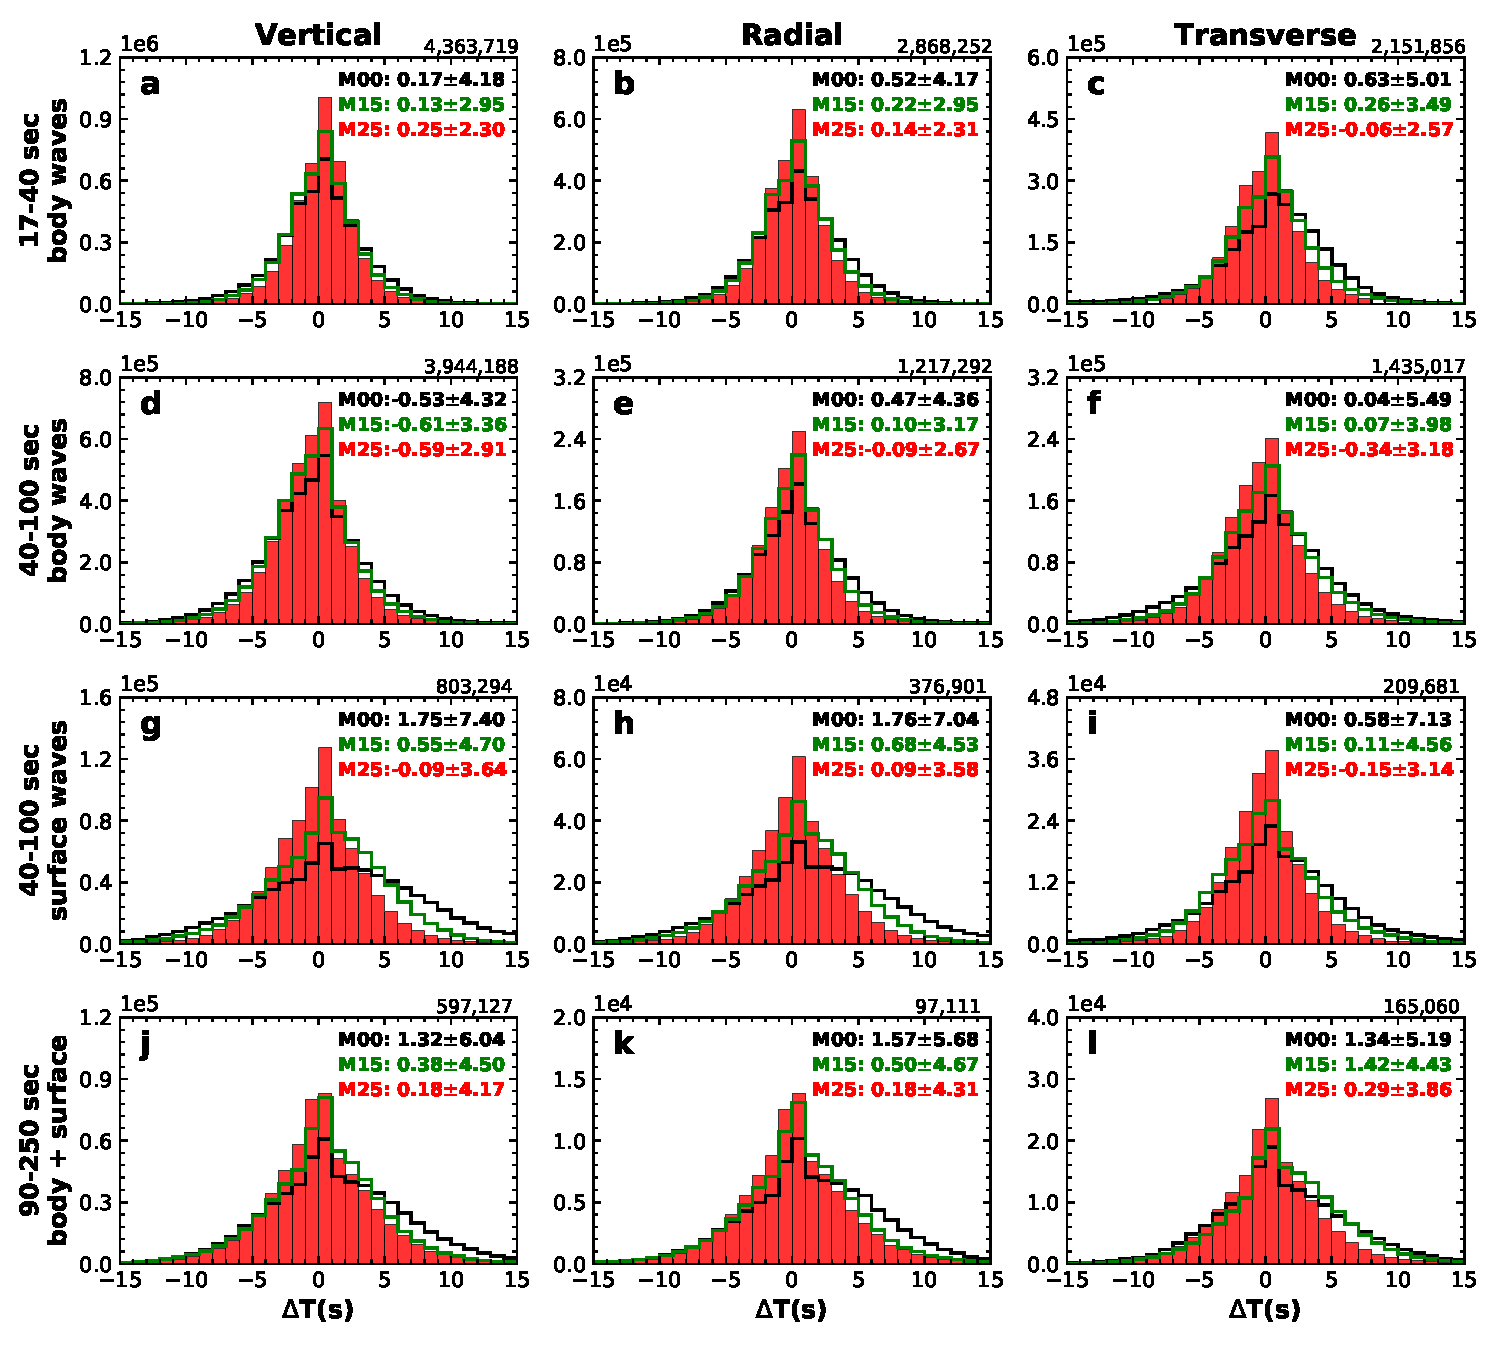
\includegraphics[width=\textwidth]{figures/dt_histogram.pdf}
\caption{Histogram of travel-time measurements from 1480 earthquakes.}
\centering
\end{figure}

\begin{figure}
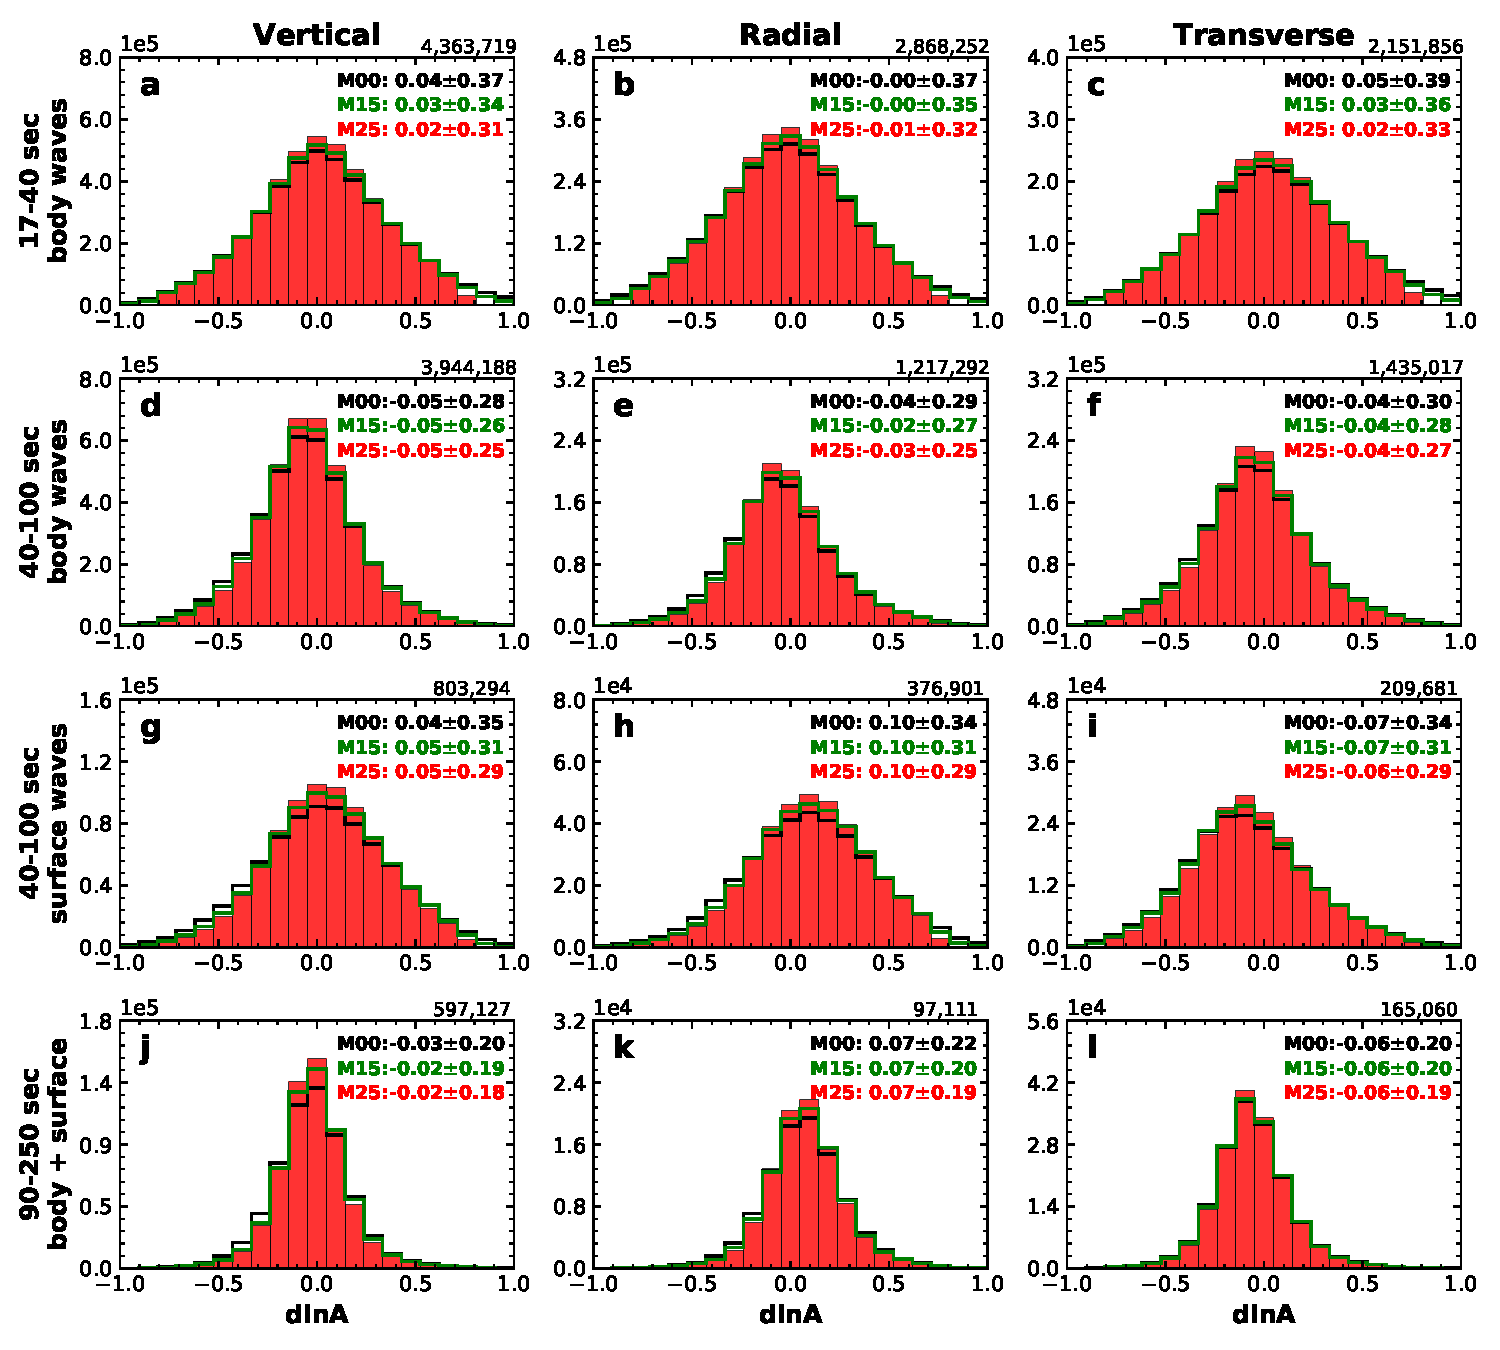
\includegraphics[width=\textwidth]{figures/dlna_histogram.pdf}
\caption{Histogram of travel-time measurements from 1480 earthquakes.}
\centering
\end{figure}

Also include the P arrival measurements here.

\begin{figure}
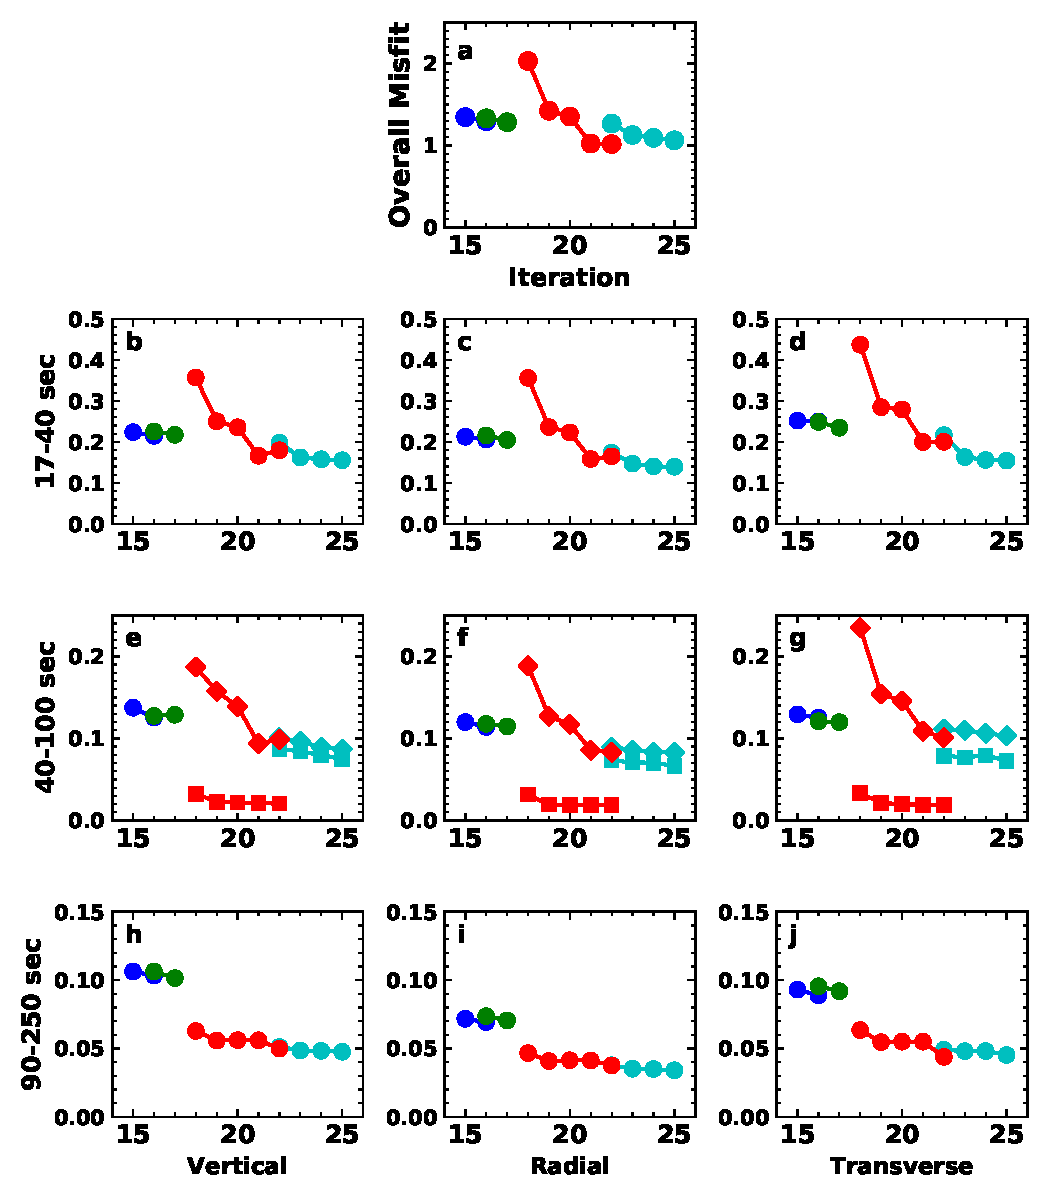
\includegraphics[width=\textwidth]{figures/misfit.pdf}
\caption{Misfit Changes from GLAD-M15 to GLAD-M25}
\centering
\end{figure}


\section{Models}

\subsection{Depth cross-section}

\begin{figure}
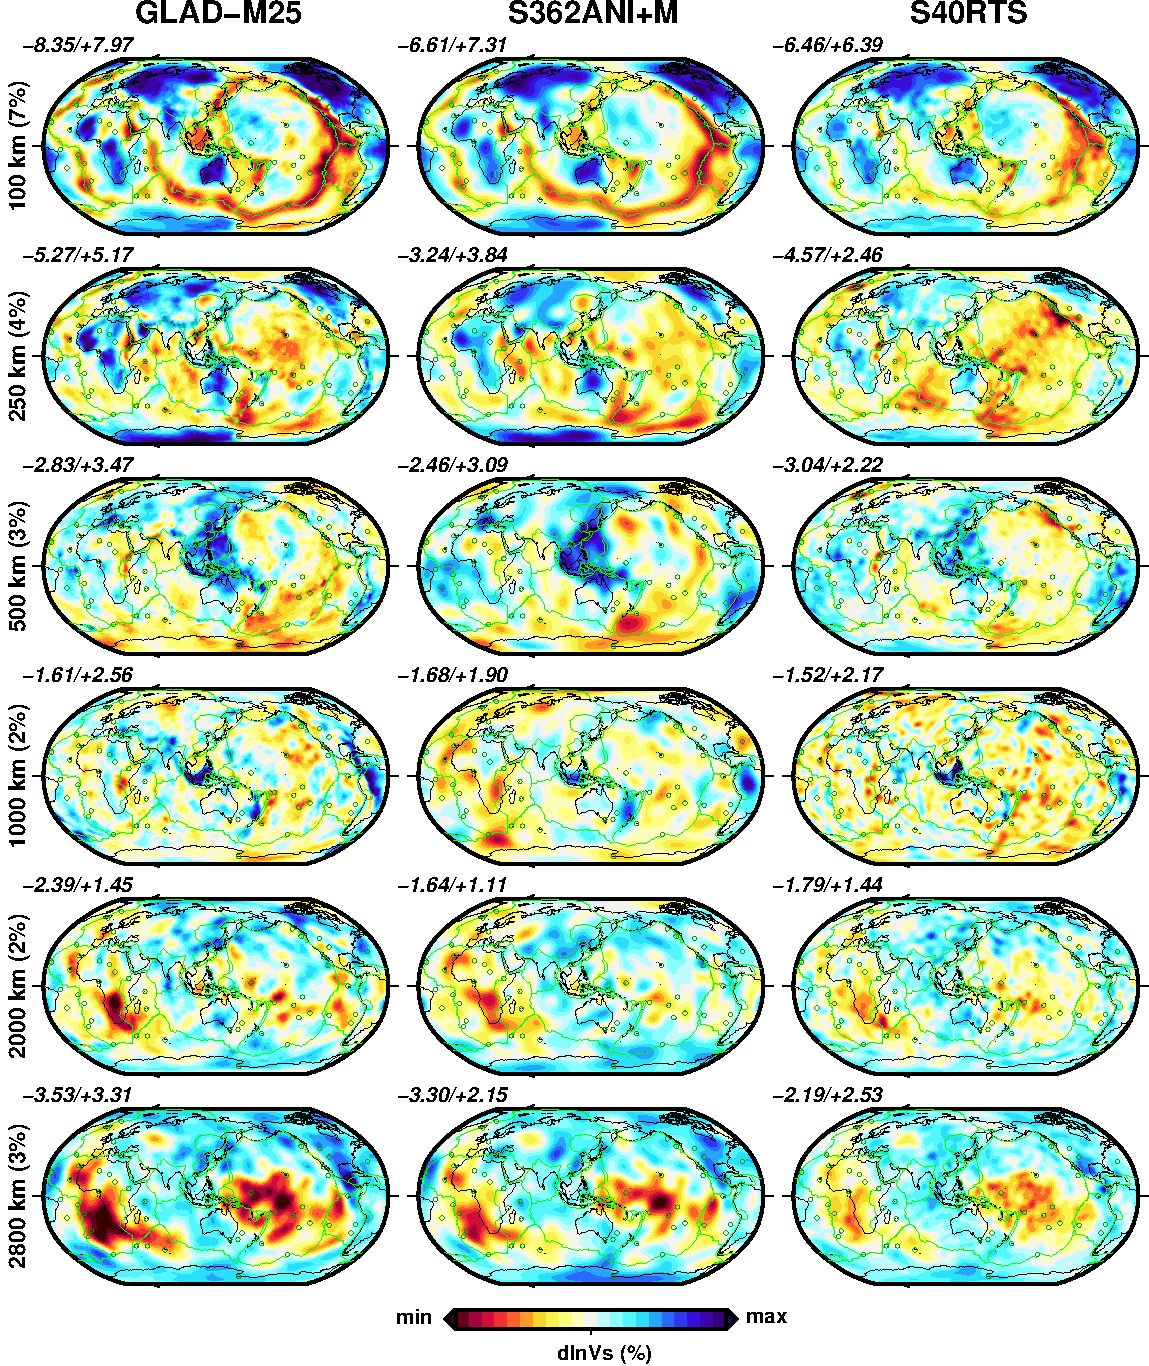
\includegraphics[width=0.9\textwidth]{figures/depth_slice/globe_vs.pdf}
\caption{Map views of global $V_s$ perturbations at various depths for out model GLAD-M25(left column), S362ANI+M(middle column)\cite{} and S40RTS\cite{}. The perturbations are calculated based on each model's own 1D profile. The values(upper-left corner of each figure) denotes the minimum/maximum perturbations for each model at the corresponding depth. The green circles denotes the locations of hotspots\cite{}. The range of the colorbar is the same for each row and the range value is labeled on the most left, right after the depth.}
\label{fig:global-vs}
\centering
\end{figure}

\begin{figure}
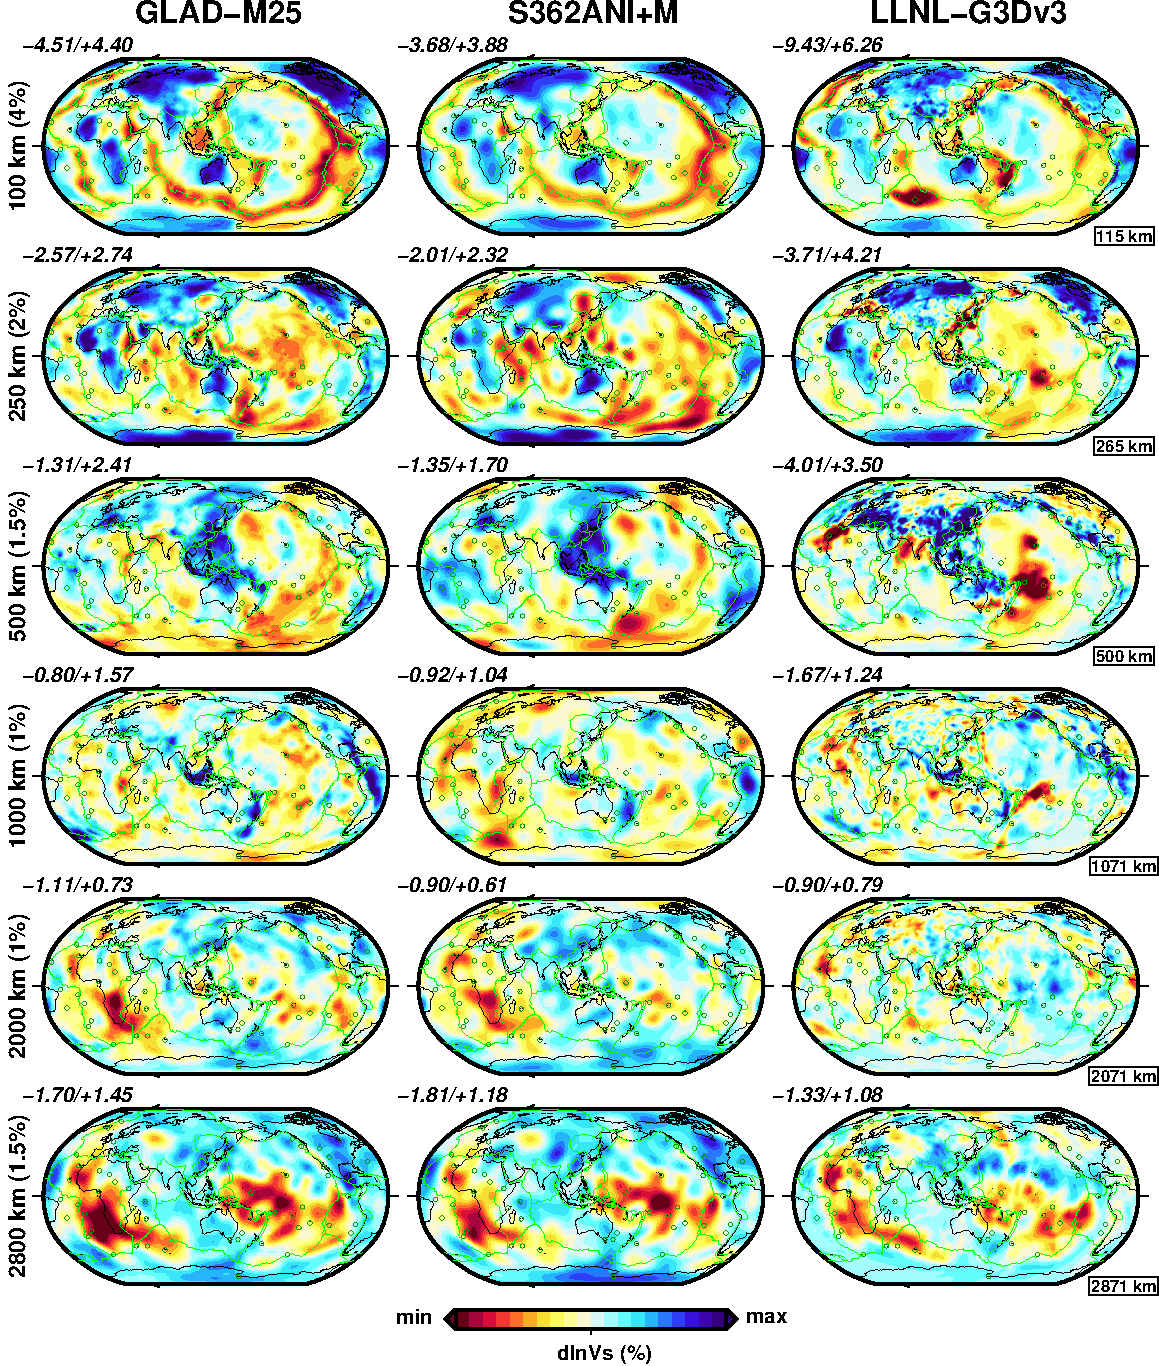
\includegraphics[width=0.9\textwidth]{figures/depth_slice/globe_vp_S362ANI-LLNL.pdf}
\caption{Map views of global $V_p$ variations at various depths for our model GLAD-M25(left column), S362ANI+M(middle column) and LLNL-G3Dv3\cite{}. For LLNL-G3Dv3, the depths is labeled on the right bottom due to its specific mesh spacing. Other plotting conventions are used similar as in Figure \ref{fig:global-vs}.}
\label{fig:global-vp}
\centering
\end{figure}

\begin{figure}
\centering
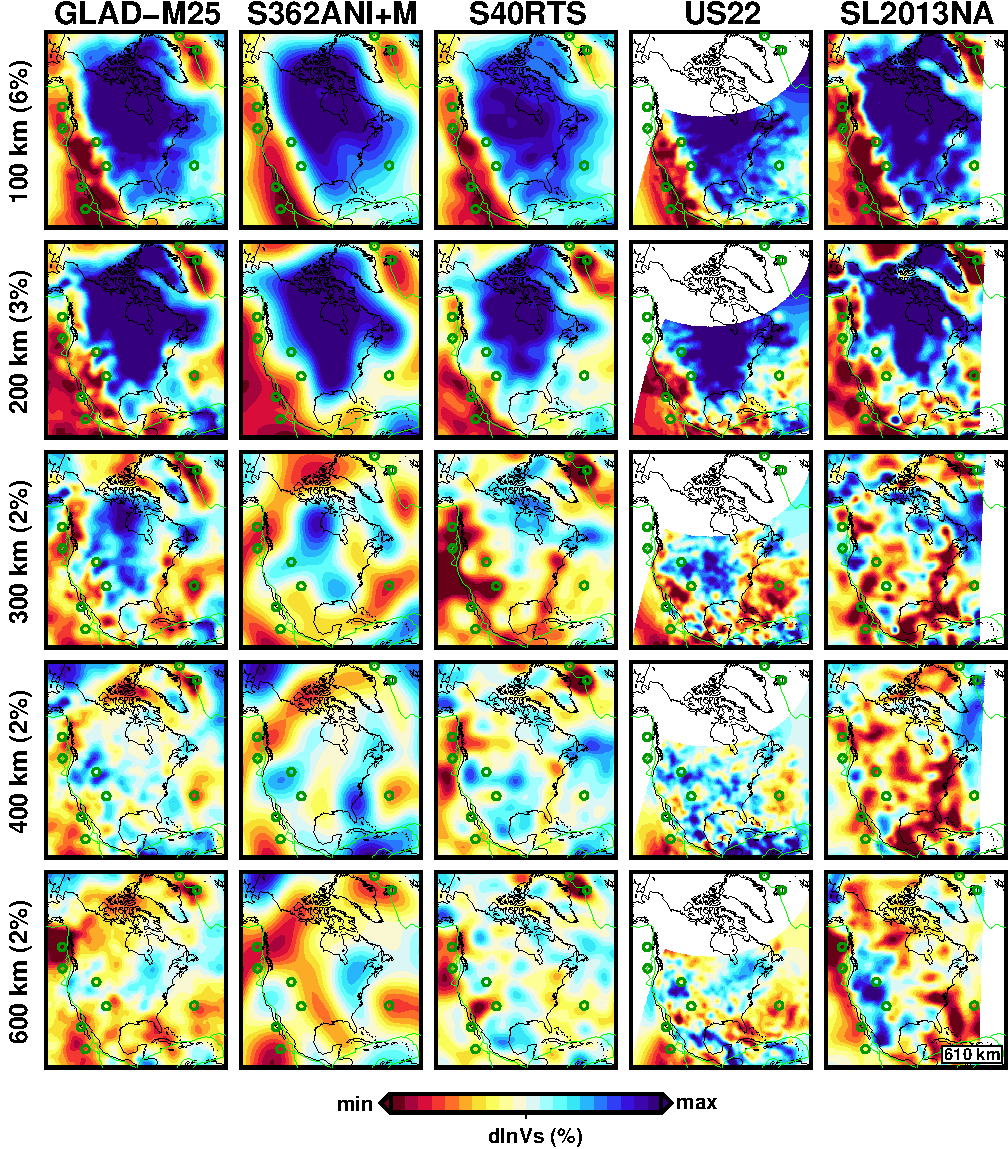
\includegraphics[width=0.9\textwidth]{figures/depth_slice/america_vs.pdf}
\caption{Map views of $V_s$ variations of North America at various depths for our model GLAD-M25(first column) and several global(S362ANI+M and S40RTS) and regional(US22 and SL2013NA) models. \ref{fig:global-vs}. Green circles denotes the locations of hotspots. For SL2013NA, we showed the 610km instead of 600km due to its own mesh grid.}
\label{fig:global-vp}

\end{figure}

\begin{figure}
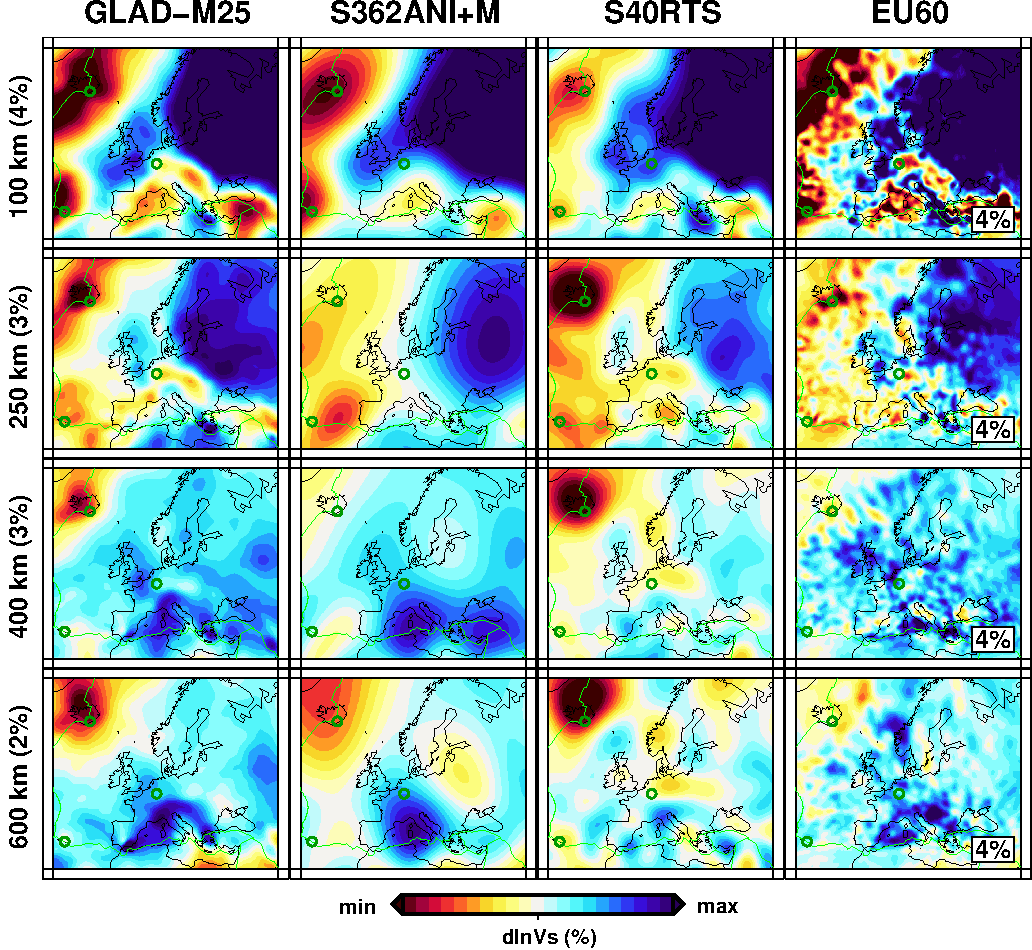
\includegraphics[width=0.9\textwidth]{figures/depth_slice/europe_vs.pdf}
\caption{Map views of $V_s$ variations of Europe at various depths for our model GLAD-M25(first column) and global(S362ANI+M and S40RTS) and regional(EU60) models. For EU60, the range of color bar is 4\% for all depths, which is labeled in the right bottom corner of the figures.}
\label{fig:global-vp}
\centering
\end{figure}


\begin{figure}
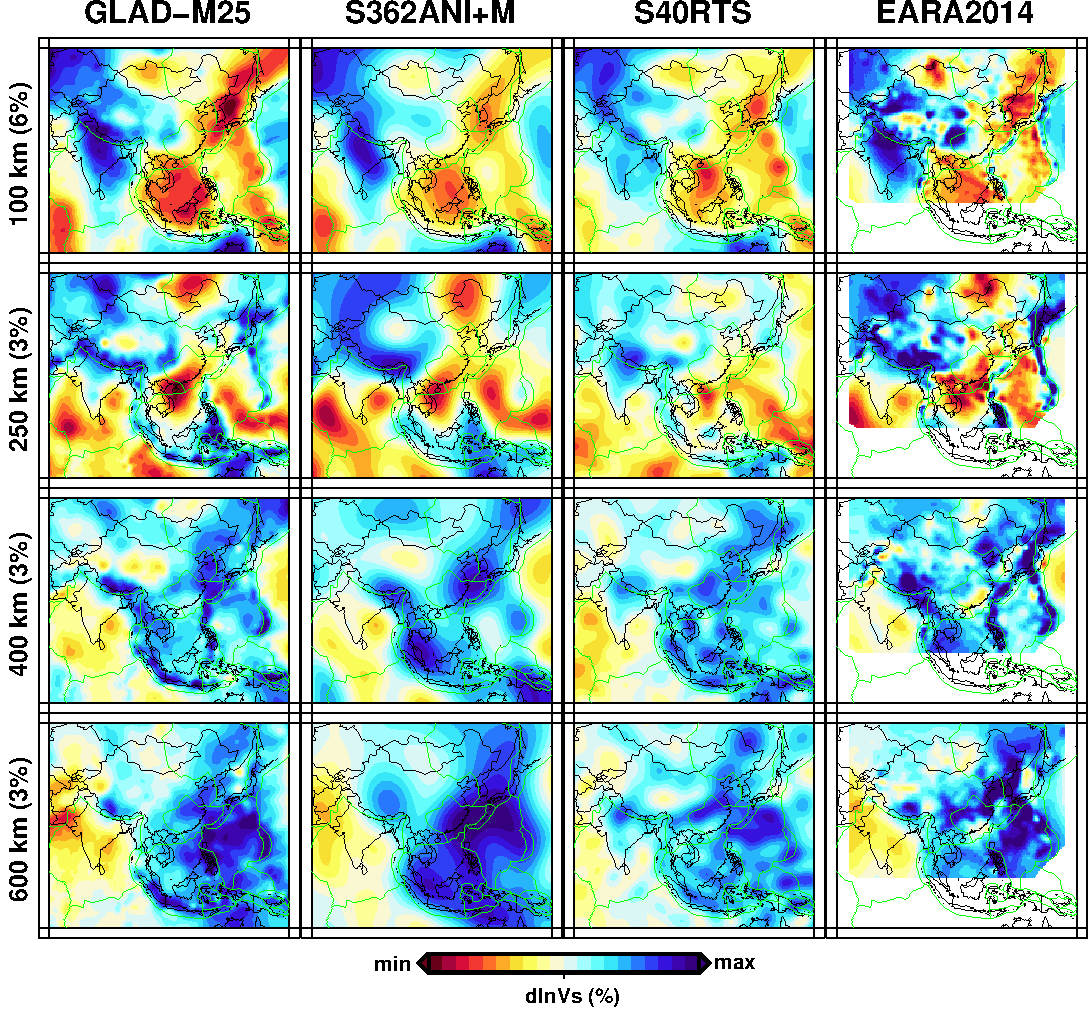
\includegraphics[width=0.9\textwidth]{figures/depth_slice/asia_vs.pdf}
\caption{Map views of $V_s$ variations of Asia at various depths for our model GLAD-M25(first column) and several global(S362ANI+M and S40RTS) and regional(EARA2014) models.}
\label{fig:global-vp}
\centering
\end{figure}


\begin{figure}
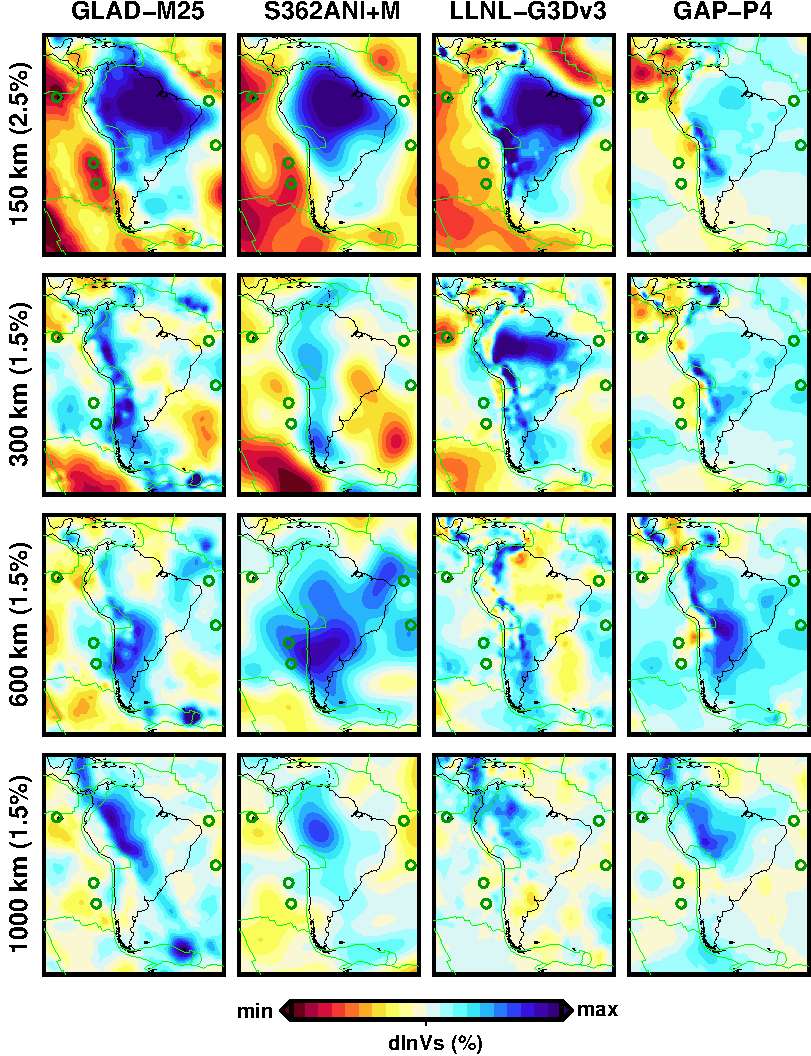
\includegraphics[width=0.9\textwidth]{figures/depth_slice/south_america_vp.pdf}
\caption{Map views of $V_p$ variations of Europe at various depths for our model GLAD-M25(first column) and several global models, including S362ANI+M, LLNL-G3Dv3 and GAP-P4.}
\label{fig:global-vp}
\centering
\end{figure}

\subsection{Plumes}

%\begin{figure}[h]
%    \centering
%    \sidesubfloat[]{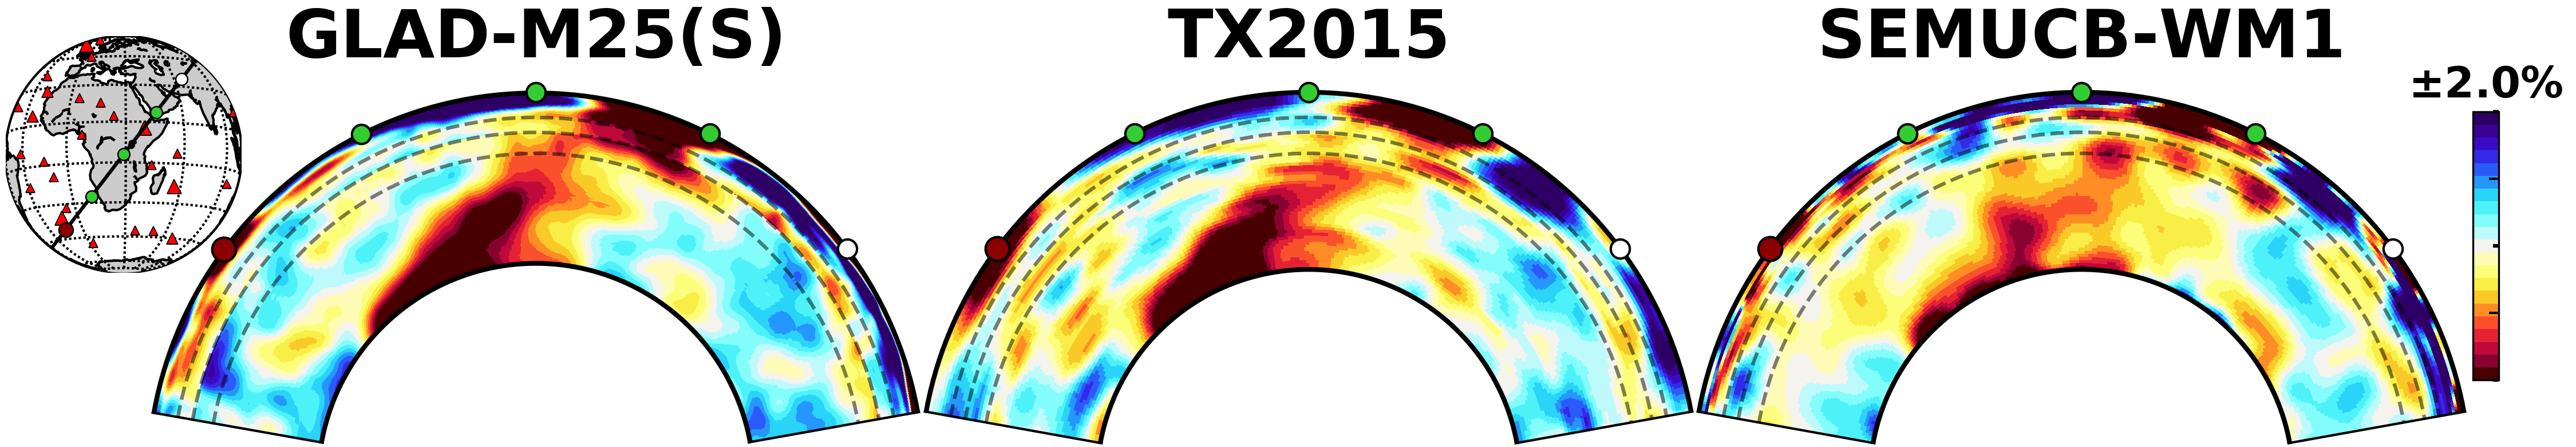
\includegraphics[width=0.98\textwidth]{figures/plumes/Afar.png}\label{fig:a}}\\[-1pt]
%    \sidesubfloat[]{
\includegraphics[width=0.98\textwidth]{figures/plumes/Bermuda_Canary.png}\label{fig:b}}\\[-1pt]
%    \sidesubfloat[]{
\includegraphics[width=0.98\textwidth]{figures/plumes/CapeVerde_Hoggar.png}\label{fig:c}}\\[-1pt]
%    \sidesubfloat[]{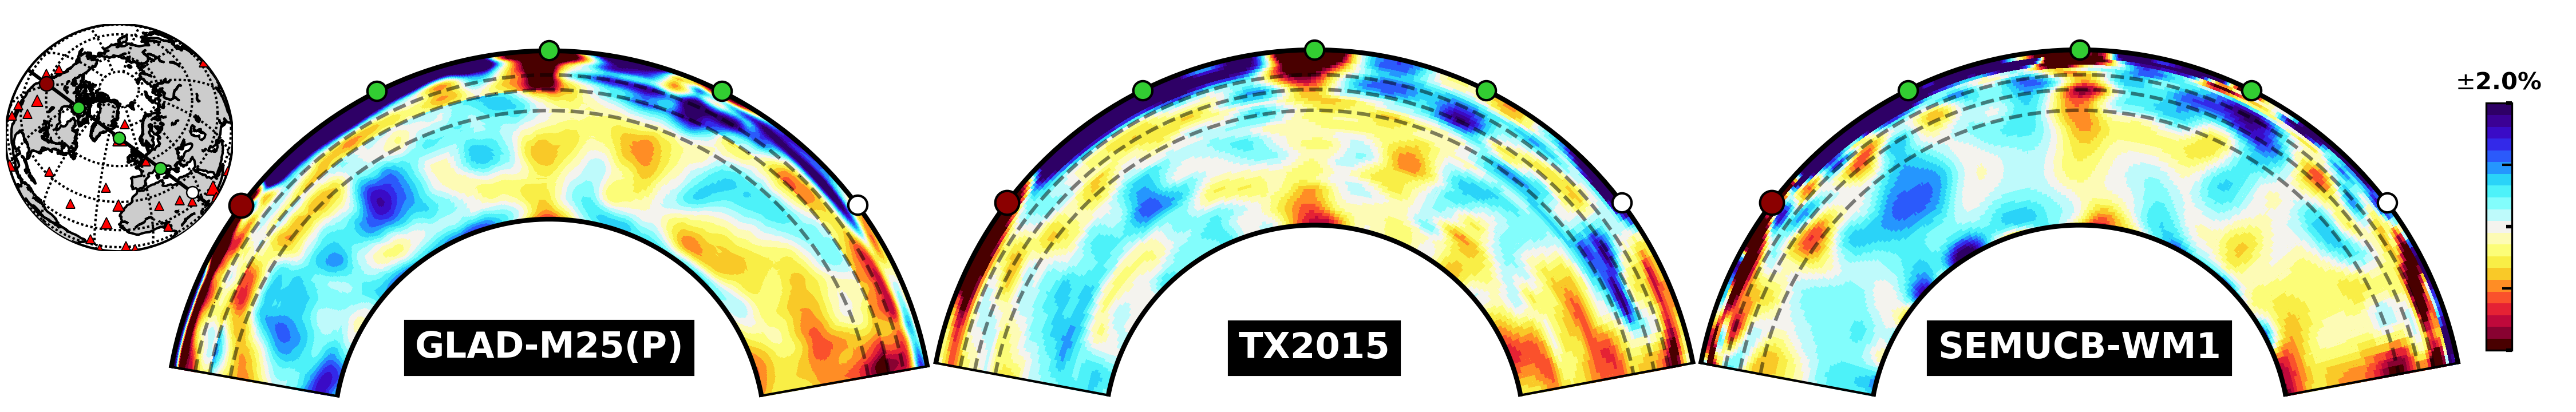
\includegraphics[width=0.98\textwidth]{figures/plumes/Iceland_Eifel.png}\label{fig:d}}\\[-1pt]
%    \sidesubfloat[]{
\includegraphics[width=0.98\textwidth]{figures/plumes/Canary_Iceland.png}\label{fig:e}}\\[-1pt]
%    \sidesubfloat[]{
\includegraphics[width=0.98\textwidth]{figures/plumes/Hoggar_AFAR.png}\label{fig:f}}\\[-1pt]
%    \sidesubfloat[]{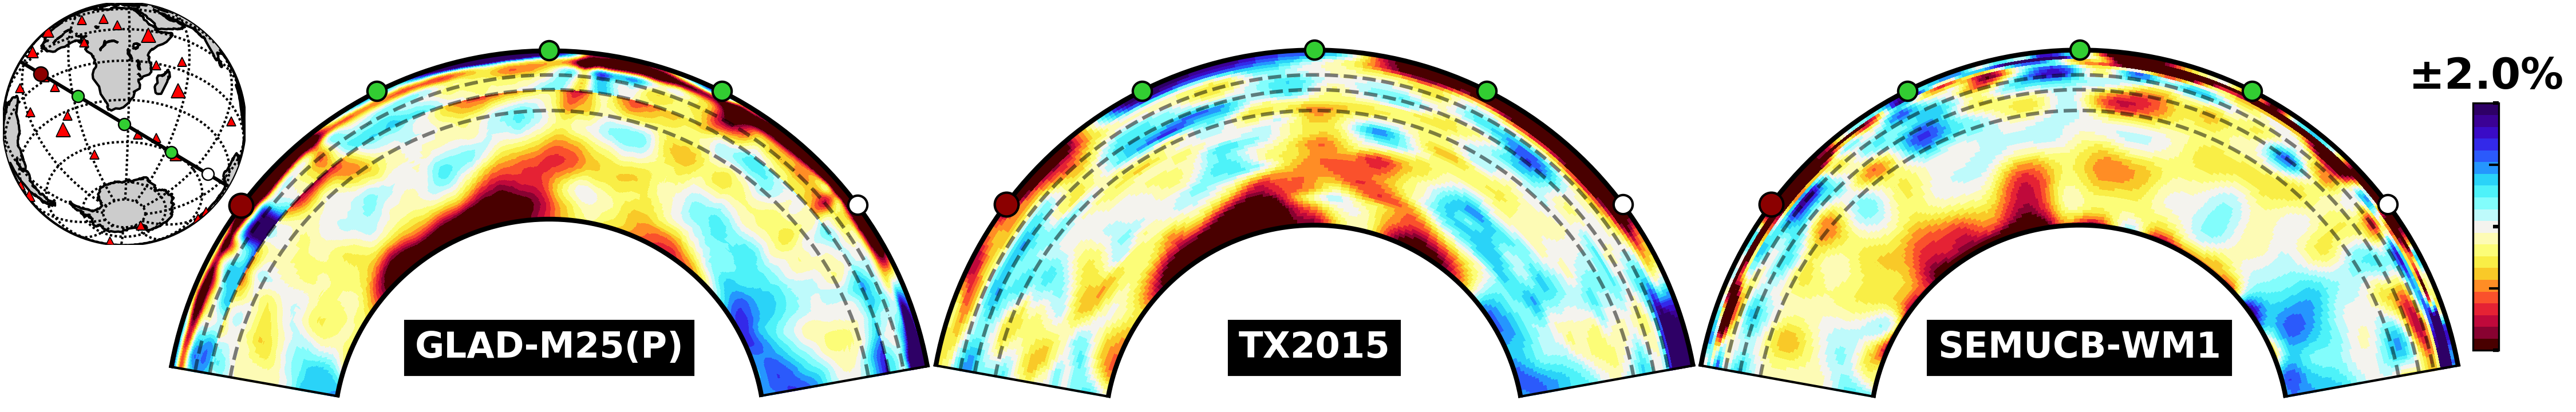
\includegraphics[width=0.98\textwidth]{figures/plumes/Marion3_Kerguelen.png}\label{fig:g}}\\
%    \caption{Vertical cross sections of perturbations of shear wave velocity Vs of plumes near the AFAR region.}
%\end{figure}

%\begin{figure}[h]
%    \centering
%    \sidesubfloat[]{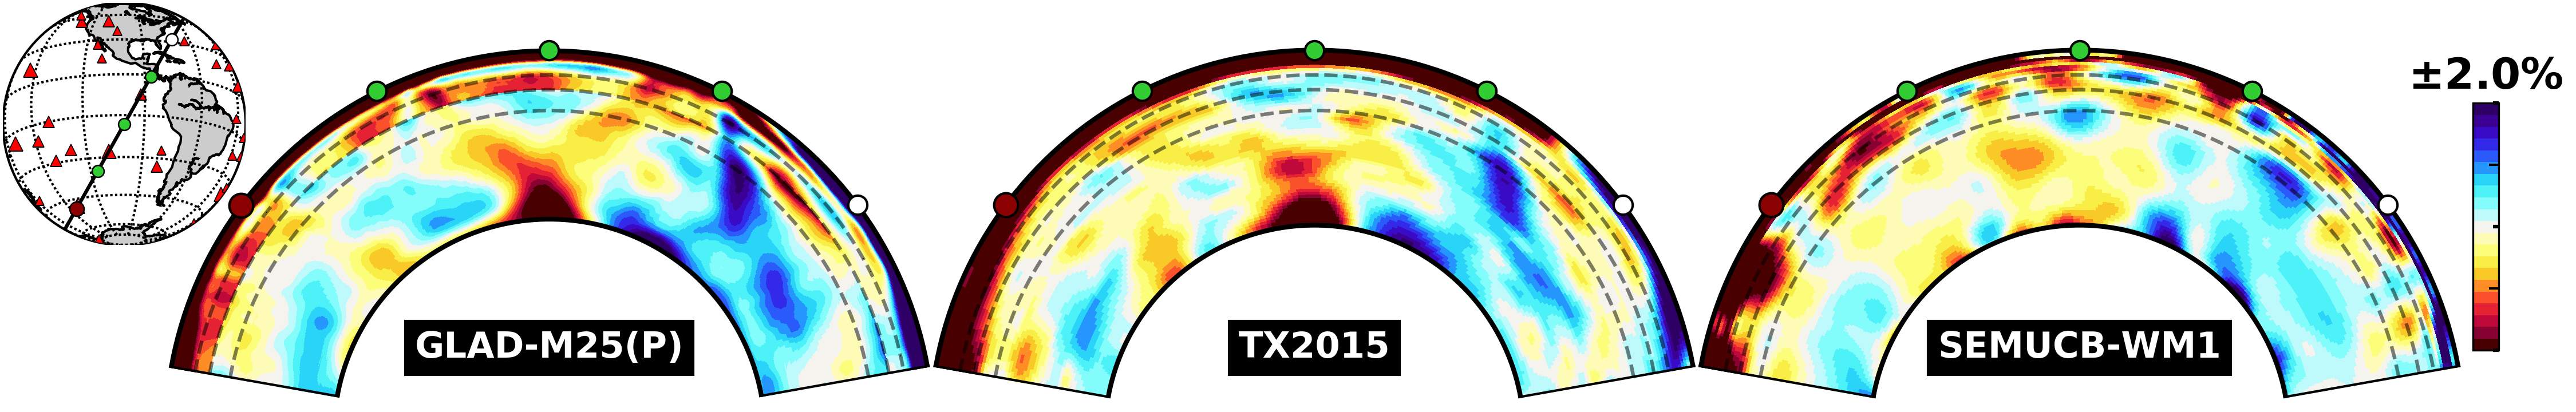
\includegraphics[width=0.98\textwidth]{figures/plumes/Easter_Galapagos.png}\label{fig:a}}\\[-1pt]
%    \sidesubfloat[]{
\includegraphics[width=1.0\textwidth]{figures/plumes/Macdonald_Yellowstone.png}\label{fig:b}}\\[-1pt]
%    \sidesubfloat[]{
\includegraphics[width=1.0\textwidth]{figures/plumes/Pitcairn_Guadalupe.png}\label{fig:c}}\\[-1pt]
%    \sidesubfloat[]{
\includegraphics[width=1.0\textwidth]{figures/plumes/Samoa_Hawaii.png}\label{fig:d}}\\[-1pt]
%    \sidesubfloat[]{
\includegraphics[width=1.0\textwidth]{figures/plumes/Samoa_MarquesasS1.png}\label{fig:e}}\\[-1pt]
%    \sidesubfloat[]{
\includegraphics[width=1.0\textwidth]{figures/plumes/Tahiti_Macdonald.png}\label{fig:f}}\\
%    \caption{Vertical cross sections of shear wave velocity perturbations of plumes in the pacific region.}
%\end{figure}

\subsection{Subductions}

\section{Model Assesement}

\subsection{Out-of-Sample Test}

The goal is to picked unseen events and check the performance of our model using those events. We revisited the Global CMT catalogue, picked the events whose magnitude is between 6.3 and 7.0. There are in total of 360 earthquakes we choosed based. We calibrated the scalar moment and origin time in the GLAD-M25 and luanched forward simulations in variaous stage of GLAD models. 

\begin{figure}
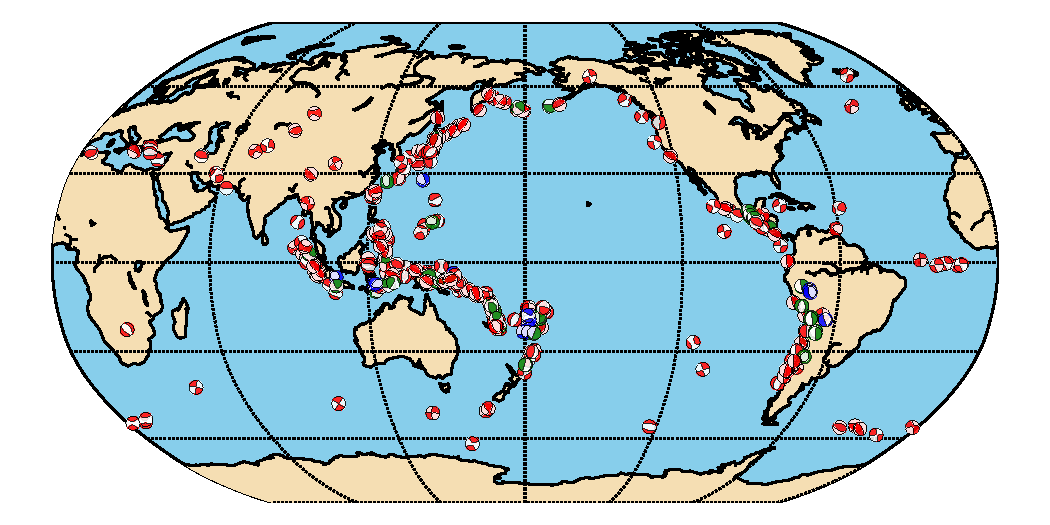
\includegraphics[width=\textwidth]{figures/events_360.pdf}
\caption{Locations of 360 out-of-sample earthquakes used in the model assessment stage.}
\centering
\end{figure}

\begin{figure}
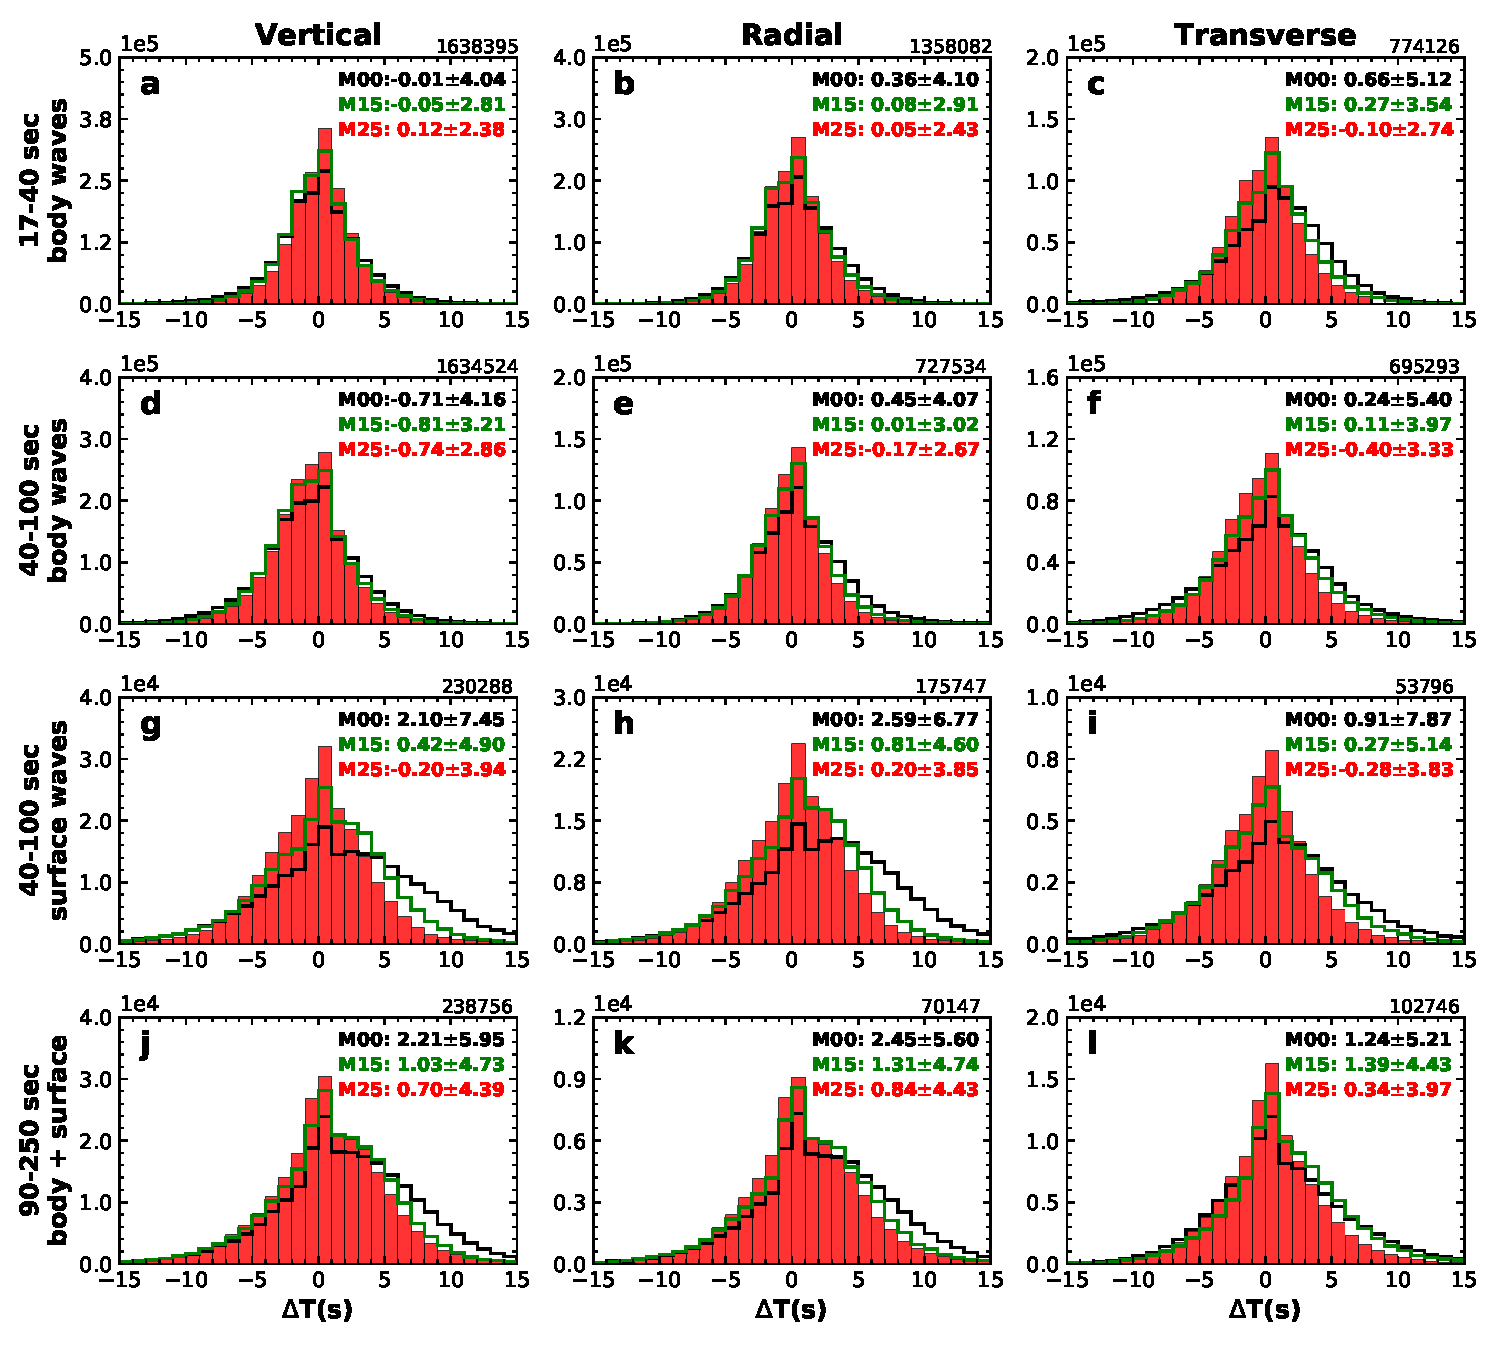
\includegraphics[width=\textwidth]{figures/dt_histogram_360.pdf}
\caption{Histogram of travel-time measurements from out-of-sample earthquakes.}
\centering
\end{figure}

\subsection{Resolution Test}


\section{Conclusion}


\begin{acknowledgments}
thanks blabla...
\end{acknowledgments}

\cite{zhu2012structure}

\newpage

\bibliographystyle{gji}
\bibliography{ref.bib}
  
\end{document}

